\chapter{Analisi idrologica e idraulica dell’area allo stato di fatto (valutazione del deflusso in SWMM)}\label{cap:progettoBase}
Prima di passare all'utilizzo di SWMM si è deciso quali metodologie usare all'interno dello studio.
Per la depurazione delle piogge si applica il metodo del Curve Number ($CN$) basato su Green-Ampt. 
Questo metodo utilizza le informazioni fornite dal Soil Conservation Service ($SCS-CN$), cioè il volume netto totale di un evento di pioggia e le perdite iniziali, per calibrare due parametri del modello di Green-Ampt ($GA$), ossia il tempo di "stagno (ponding)" e la conducibilità idraulica satura del suolo.
Questo metodo è vantaggioso in quanto per essere applicato richiede solamente la stima del Curve Number ($CN$) e della conducibilità idraulica ($K_s$). 
Il $CN$ si classifica in funzione del tipo e uso del suolo. 

Inoltre si valutano le portate delle condotte attraverso il modello di simulazione afflussi-deflussi e il modello di propagazione idraulica all'interno della rete nel software SWMM.

I due modelli sopra citati, per valutare i processi naturali, suddividono la zona in 3 comparti:
\begin{itemize}
\item \emph{atmosferico}, che rappresenta la precipitazione sul bacino urbano;
\item \emph{sottobacini}, creati da noi per suddividere l'area in partizioni che ricevono le acque dal comparto precedente e le indirizzano nel comparto \emph{rete di trasporto} come ruscellamento superficiale;
\item \emph{rete di trasporto}, che rappresenta l'insieme della rete: canali, tubi, vasche e LID.
\end{itemize}
A questo punto, dopo aver individualizzato le metodologie da utilizzare, si passa allo svolgimento dell'analisi idrologica e idraulica dell'area allo stato di fatto con il fine di valutare il deflusso della zona di studio.
Per elaborare queste analisi si impiega il software SWMM impostando un primo "progetto di base" per valutare i dati preliminari attraverso un modello cinematico.

Inizialmente si utilizza la figura \ref{fig:sottobacini} come sfondo su SWMM per il progetto di base andando ad inserire le coordinare che si sono ricavate precedentemente da QGIS.
Con l'aiuto dello sfondo si riportano i sottobacini inserendo in ognuno i dati in precedenza dedotti, come l'area totale, la percentuale di area impermeabile, la pendenza media e la larghezza di drenaggio calcolata come rapporto tra area [\si{\square\metre}] e lunghezza di drenaggio media [\si{\metre}] (Vedi Tabella \ref{tab:dati}).

\begin{table}[htb]
    \centering
    \caption{Dati dei sottobacini ricavati da QGIS da inserire in SWMM.}
    \label{tab:dati}
    \begin{tabular}{cS[table-format=1.4]S[table-format=3.0]S[table-format=3.2]S[table-format=1.2]}
        \toprule
        \multicolumn{1}{c}{\multirow{3}{*}{Sottobacino}} & \multicolumn{1}{c}{Area}&\multicolumn{1}{c}{Area}&\multicolumn{1}{c}{Larghezza}&\multicolumn{1}{c}{Pendenza}\\
        & \multicolumn{1}{c}{Totale}&\multicolumn{1}{c}{Impermeabile}&\multicolumn{1}{c}{Drenaggio}&\multicolumn{1}{c}{Media}\\
        & \multicolumn{1}{c}{[\si{\hectare}]} & \multicolumn{1}{c}{[\si{\percent}]}&\multicolumn{1}{c}{[\si{\metre}]}&\multicolumn{1}{c}{[\si{\percent}]}\\
        \midrule
01        & 0.3016      & 37                & 54.18               & 2.96           \\
02        & 0.6697      & 96                & 150.49              & 1.25           \\
03        & 0.3430      & 64                & 86.47               & 0.70           \\
04        & 0.5204      & 32                & 81.74               & 2.57           \\
05        & 0.3233      & 41                & 50.25               & 2.88           \\
06        & 0.9783      & 76                & 138.44              & 1.87           \\
07        & 0.8352      & 90                & 129.49              & 1.08           \\
08        & 0.7659      & 73                & 153.18              & 1.18           \\
09        & 0.3640      & 10                & 65.00               & 3.77           \\
10       & 0.6387      & 43                & 109.31              & 2.28           \\
11       & 0.5152      & 82                & 78.86               & 1.62           \\
12       & 0.3768      & 9                 & 63.86               & 3.99           \\
13       & 0.4092      & 6                 & 77.21               & 2.75           \\
14       & 0.3311      & 14                & 57.83               & 1.40           \\
15       & 0.8532      & 76                & 109.85              & 1.70           \\
16       & 0.4011      & 10                & 55.71               & 3.25           \\
17       & 0.4547      & 7                 & 60.43               & 1.29           \\
18       & 0.3676      & 83                & 59.77               & 2.18           \\
19       & 0.3808      & 27                & 61.82               & 2.84           \\
20       & 0.5283      & 77                & 93.09               & 2.03           \\
21       & 0.7326      & 82                & 93.03               & 1.89           \\
22       & 3.1032      & 100               & 197.66              & 1.59           \\
23       & 1.3079      & 70                & 108.09              & 1.21           \\
24       & 1.6037      & 85                & 187.93              & 1.16           \\
25       & 1.3684      & 79                & 139.07              & 0.93           \\ \bottomrule
\end{tabular}
\end{table}

Successivamente si costruiscono degli ietogrammi che rappresentano l'andamento dell'intensità di pioggia per una determinata durata. 
Prima si valuteranno degli ietogrammi costanti per una prima analisi grossolana e per ricavare il tempo critico.
Infine, con l'analisi dei precedenti ietogrammi, si passerà alla realizzazione del ietogramma Chicago per una rappresentazione più dettagliata e precisa dell'andamento dell'intensità di precipitazione.
% Infatti con l'inserimento di quest'ultimo ietogramma si passa dal progetto di base al progetto vero e proprio andando ad inserire su SWMM la rete di drenaggio ipotizzata su QGIS.(Fig. bo una con rete)
% In questa fase progettuale con i modelli di simulazione afflussi-deflussi e di propagazione idraulica all'interno della rete si progettano e verificano le condotte, cioè il diametro, il riempimento, l'autopulizia e la velocità dell'acqua, sistemi di laminazione puntuali, come le vasche volano, e sistemi diffusi, come i LID. 

% QUA SE VUOI AMPLIARE UN PO TE CHE STAI FACENDO QUESTA PARTI ALTRIMENTI LASCIAMO COSì O VALUTIAMO INSIEME.

% https://www.researchgate.net/publication/308697020_METODI_MISTI_DI_DEPURAZIONE_DELLA_PIOGGIA_BASATI_SUL_CURVE_NUMBER
\section{Caratteristiche dell’area allo stato di fatto}
Tenendo in considerazione la metodologia di depurazione delle acque si procede al calcolo del $CN$. 
Per fare ciò si considera una massima capacità di ritenzione idrica del suolo $S$ compresa tra \SI{85} e \SI{162}{\milli\metre} e dalla formula \ref{eq:CN} si ottiene un $CN$ tra \SI{74.92} e \SI{61.06}.
\begin{equation}
\label{eq:CN}
    CN = \frac{\SI{25400}{}}{\SI{254}{} + S}
\end{equation}
Si è deciso di applicare di applicare il valore massimo di $CN$ pari a \SI{74.92}.

Considerando che il terreno dell'area di studio sia principalmente sabbioso e con tratti ghiaiosi e limosi, attraverso la tabella 4-7 di SWMM riportata nell'appendice \ref{appendix:SWMM} a pagina \pageref{SWMM:tabella4-7} si sono scelti due parametri di conduttività idraulica $K_s$: \SI{0.43} per una classe di terreno \emph{terriccio sabbioso} e \SI{1.18} per una classe \emph{sabbia limosa}. 
Per la seguente relazione si è deciso di tener conto di un terreno con classe \emph{terriccio sabbioso}.

Infine si è proceduto al calcolo del tempo di secca $T_{\text{secco}}$, cioè il periodo di tempo che impiega il suolo completamente saturo a tornare allo stato secco.
Questo perché per la simulazione continua in SWMM richiede di specificare una stima del tempo di secca in giorni.
Utilizzando il metodo di Green-Ampt questo tempo si basa esclusivamente sulla conducibilità idraulica $K_s$ e la sua stima si calcola con la formula: 
\begin{equation}
    T_{\text{secco}} = \frac{\SI{3.125}{}}{\sqrt{K_s}}
\end{equation}
dove $K_s$ è espresso in \si{in\per\hour}.
Nel nostro caso si ha che risulta pari a \SI{4.76}{\days} per \emph{terriccio sabbioso} e \SI{2.88}{\days} per \emph{sabbia limosa}. 
Quindi in base alla classe di terreno scelta precedentemente, si è preso in considerazione il valore di \SI{4.76}{\days}.

Dopodiché per ciascuno di questi si è valutato solamente un recapito finale posto nel rivo Adigetto nella parte sud di Via Roberto da Sanseverino. 
Facendo così tutti i sottobacini creati avranno lo stesso scarico di deflusso (Figura \ref{fig:ProgettoBase}).
\begin{figure}[p]
    \centering
    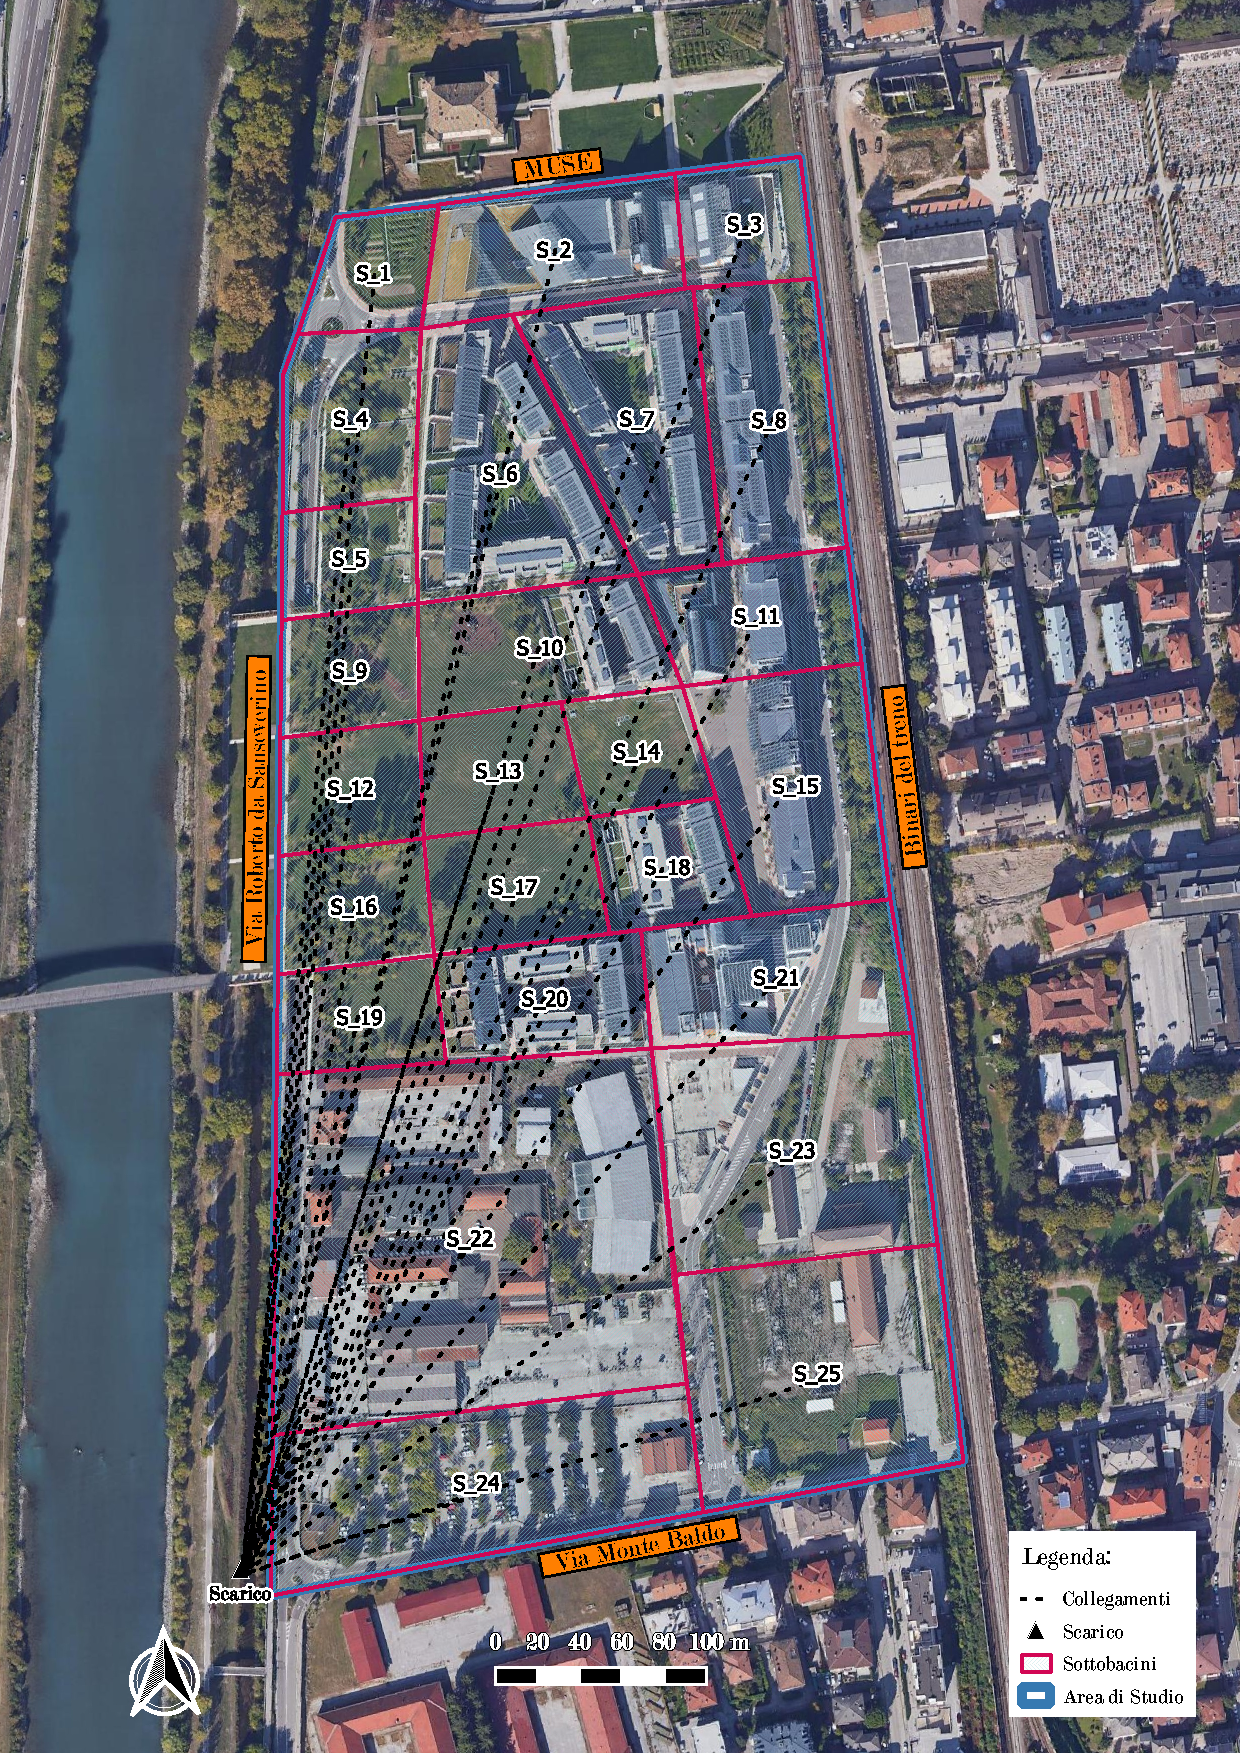
\includegraphics[trim=0cm 0cm 0cm 0cm,clip,frame,width=0.9\textwidth]{IMG/ProgettoBase.pdf} 
    \caption{Posizionamento del recapito finale per verificare il deflusso dei sottobacini}
    \label{fig:ProgettoBase}
\end{figure}

Questo, come vedremo nel paragrafo successivo, ci sarà utile per la valutazione del tempo critico del bacino.

\section{Ietogramma di progetto}
Gli ietogrammi di progetto rappresentano l'andamento dell'intensità di pioggia per tutta la sua durata. Per una prima analisi grossolana si sono utilizzati ietogrammi costanti. Per elaborare i seguenti grafici si assegna un determinato tempo di ritorno, nel caso in esame pari a 25 anni, e una durata della pioggia $t_p$. 
Questi ietogrammi si eseguono per la valutazione del tempo critico del bacino urbano. Dai parametri $a$ e $n$ delle curve di possibilità pluviometriche, ricavati nel capitolo 2, si deduce l'intensità di precipitazione $i$ che viene tenuta costante per tutta la durata di pioggia dell'evento. L'intensità si ricava dalla seguente espressione:
\begin{equation}
    i = a \, t_p ^{n - 1}
\end{equation}
dove per $t_p$ si intende la durata espressa in ore. 
Si riportano in tabella \ref{tab:ietocost} i valori delle intensità di pioggia per ogni durata presa in considerazione.
\begin{table}[htbp]
    %\small
    \centering
    \caption{Intensità di precipitazione in funzione della durata}
    \label{tab:ietocost}
    \begin{tabular}{S[table-format=3.0]S[table-format=1.2]S[table-format=3.4]}
        \toprule
        \multicolumn{1}{c}{Durata} & \multicolumn{1}{c}{Durata} & \multicolumn{1}{c}{Intensità $i$}\\
        \multicolumn{1}{c}{[\si{\minute}]} & \multicolumn{1}{c}{[\si{\hour}]} & \multicolumn{1}{c}{[\si{\milli\metre\per\hour}]}\\
        \midrule
1 & 0.02 & 441.2547 \\
2 & 0.03 & 287.1642 \\
5 & 0.08 & 162.7469 \\
7 & 0.12 & 132.1150 \\
10 & 0.17 & 105.9141 \\
15 & 0.25 & 82.3804 \\
30 & 0.50 & 53.6123 \\
45 & 0.75 & 41.6999 \\
60 & 1.00 & 34.8904 \\
120 & 2.00 & 22.7063 \\
180 & 3.00 & 17.6611 \\
240 & 4.00 & 14.9275 \\
300 & 5.00 & 13.1951 \\ \bottomrule
\end{tabular}
\end{table}

Ci si è fermati ad un tempo di quattro ore perché oltre le tre ore e mezza, come visto nel capitolo \ref{cap:pluviometriche}, gli scrosci hanno meno importanza delle precipitazioni orarie.
Dopo aver calcolato i valori delle intensità, si prosegue sul programma SWMM.

Per iniziare sul progetto di base con lo scarico comune per ogni sottobacino si inseriscono i valori di intensità di precipitazione per ciascun ietogramma costante che si vuole realizzare e analizzare per valutare quale sia l'evento più gravoso e quindi il tempo critico del bacino. 
Dopodiché impostando nel pluviometro lo ietogramma costante e la rispettiva durata eseguendo il programma si ricevono i dati di picco di deflusso, di infiltrazione, di deflusso totale e di quantità di precipitazione.
Quest'ultima si può verificare facilmente dato che corrisponde all'intensità di pioggia moltiplicata per il rispettivo tempo di durata.

Ottenuti tutti i dati degli ietogrammi costanti si analizza il deflusso di ciascuno andando a constatare quale curva dia il picco maggiore e di conseguenza sapere quale sia il tempo critico del bacino (Figura \ref{fig:DeflussoBacinoIetogrammiCostanti}). 
Come si nota da questa figura il picco più gravoso e quindi l'evento meteorologico che influenza maggiormente l'area di studio si ha con una durata di pioggia di \SI{5}{\minute}.
Questo evento anche se molto breve per la nostra zona si può considerare come evento critico data la presenza di molte aree impermeabili e quindi l'area si trasforma subito in deflusso.

\begin{figure}[htb]
    \centering
    \begin{tikzpicture}
        \begin{axis}[
            restrict x to domain=-0:1.5,
            height=8cm,
            width=\textwidth,
            grid=major,
            xlabel=Tempo trascorso dall'inizio della precipitazione \si{[\hour]},
            ylabel=Deflusso  \si{[\litre\per\second]},
            xtick = {0,0.5,1,1.5,2,2.5,3,3.5,4},
            %title= ,
            /pgf/number format/.cd,
            use comma,
            1000 sep={\,}
        ]
        \addplot +[mark=none,style=solid,color=red] table[x index=0,y index=1,header=false] {IMG/Total-Inflow/total_inflow_1min.txt};
        \addplot +[mark=none,style=solid,color=green!60!black] table[x index=0,y index=1,header=false] {IMG/Total-Inflow/total_inflow_2min.txt};
        \addplot +[mark=none,style=solid,color=magenta] table[x index=0,y index=1,header=false] {IMG/Total-Inflow/total_inflow_5min.txt};
        \addplot +[mark=none,style=solid,color=cyan] table[x index=0,y index=1,header=false] {IMG/Total-Inflow/total_inflow_10min.txt};
        \addplot +[mark=none,style=solid,color=orange] table[x index=0,y index=1,header=false] {IMG/Total-Inflow/total_inflow_15min.txt};
        \addplot +[mark=none,style=solid,color=teal] table[x index=0,y index=1,header=false] {IMG/Total-Inflow/total_inflow_30min.txt};
        \addplot +[mark=none,style=solid,color=violet] table[x index=0,y index=1,header=false] {IMG/Total-Inflow/total_inflow_45min.txt};
        \legend{1 min,2 min,5 min,10 min,15 min,30 min,45 min}    
        \end{axis}
    \end{tikzpicture}
    \caption{Deflusso del bacino con l'utilizzo di ietogrammi costanti a diverse durate di pioggia. Il picco massimo è con durata di \SI{5}{\minute}}
    \label{fig:DeflussoBacinoIetogrammiCostanti}
\end{figure}

Ora per migliorare la nostra analisi dell'evento meteorologico si valuta uno ietogramma Chicago che presenta andamenti temporali non costanti e che sia di durata paragonabile o comunque maggiore all'evento critico.
Non avendo molto senso uno ietogramma Chicago pari al tempo critico di \SI{5}{\minute} dato che con un tempo così ridotto non si otterrebbero dati molto significativi, si impone una durata   $t_{\text{tot}} = \SI{2}{\hour}$, per sollecitare l'area gradualmente, e una posizione di picco $r$, che generalmente nei bacini urbani è compresa tra \SI{0.3} e \SI{0.5}, a \SI{0.5} per essere più cautelativi. 
\begin{equation}
    t_\text{picco} = {r\,t_\text{tot}}
\end{equation}
Facendo così la posizione del picco del deflusso risulterà a \SI{1}{\hour} come visibile nello ietrogramma Chicago riportato in figura \ref{fig:Chicago}.

\begin{figure}[htb]
    \centering
    \begin{tikzpicture}
        \begin{axis}[
            restrict x to domain=-0:120,
            height=6cm,
            width=\textwidth,
            grid=major,
            xlabel=Tempo trascorso dall'inizio della precipitazione \si{[\minute]},
            ylabel=Intensità di pioggia  \si{[\milli\metre\per\hour]},
            %xtick = {0,0.5,1,1.5,2,2.5,3,3.5,4},
            %title= ,
            /pgf/number format/.cd,
            use comma,
            1000 sep={\,}
        ]
        \addplot +[ybar,
            mark=none,
            enlargelimits=0.15
            style=solid,
            fill,
            color=pantone186,
            xtick=data,
            %nodes near coords,
            %nodes near coords align={vertical}
            ] 
        table[x index=0,y index=1,header=false] {IMG/Total-Inflow/chicago.txt};
        \end{axis}
    \end{tikzpicture}
    \caption{Ietogramma Chicago con $T_R = 25$ anni}
    \label{fig:Chicago}
\end{figure}   

Discretizzando lo ietogramma Chicago ad intervalli di \SI{5}{\minute}, dalla figura, si osserva una prima fase di accumulo d'acqua, dove le depressioni superficiali iniziano a colmarsi, quindi prima del picco si ha che la zona è già stata in parte sollecitata.
La costruzione del ietogramma Chicago avviene attraverso le formule dell'altezza di pioggia $h(t)$ pre e post picco e l'intensità di pioggia media $i_m$, che risulterà costante a tratti di \SI{5}{\minute}.
\begin{equation}
\label{eq:altezza}
    h(t) = 
    \begin{cases}
        r \, a \left[ \left( \frac{t_p}{r}\right)^n - \left( \frac{t_p - t}{r}\right)^n  \right] & \text{se $t < t_p$}\\
        a \left[ r \left( \frac{t_p}{r}\right)^n + (1-r)\left( \frac{t_p - t}{1 - r}\right)^n  \right] & \text{se $t > t_p$}\\
    \end{cases}
\end{equation}
\begin{equation}
\label{eq:imedia}
    i_m = \frac{h(t_\text{fin}) - h(t_\text{in})}{\Delta t}
\end{equation}
Ricavati tutti i dati necessari dello ietogramma Chicago li si riportano nel programma SWMM per ottenere i risultati dell'area di studio.

\section{Risultati dell'analisi}
%Riportare i risultati della simulazione idraulica mostrando l’idrogramma di piena in uscita dall’area di studio. Riportare in maniera esplicita il valore di colmo dell’onda di piena, il coefficiente di deflusso e il coefficiente udometrico nello stato di fatto (portata al colmo diviso area (l/s/ha). Riportare anche una breve valutazione del deflusso dei vari sottobacini.
Eseguendo la simulazione idraulica {\RED{(attraverso il metodo dell'invaso lineare????)}} con SWMM con tempo di ritorno pari a 25 anni si sono riportati i dati significativi del progetto.

Ideogramma di piena in uscita con indicazione del colmo: 

tabella summery SWMM con coeffifiente di deflusso, coeff udumetrico.
\begin{table}[htbp]
    %\small
    \centering
    \caption{Dati di afflusso del progetto di base con ietogramma Chicago}
    \label{tab:afflussobase}
    \begin{tabular}{cS[table-format=2.2]S[table-format=3.2]S[table-format=1.4]S[table-format=1.2]S[table-format=3.2]}
        \toprule
        \multirow{3}{*}{Sottobacino} & \multicolumn{1}{c}{Quantità} & \multicolumn{1}{c}{Picco} & \multicolumn{1}{c}{Area} & \multicolumn{1}{c}{Coefficiente} & \multicolumn{1}{c}{Coefficiente} \\
        & \multicolumn{1}{c}{Precipitazione} & \multicolumn{1}{c}{Deflusso} & \multicolumn{1}{c}{Totale} & \multicolumn{1}{c}{Deflusso} & \multicolumn{1}{c}{Udumetrico} \\
        & \multicolumn{1}{c}{[\si{\milli\metre}]} & \multicolumn{1}{c}{[\si{\litre\per\second}]} & \multicolumn{1}{c}{[\si{\hectare}]} & \multicolumn{1}{c}{[--]} & \multicolumn{1}{c}{[\si{\litre\per\second\per\hectare}]} \\
        \midrule
01 & 45.41 & 24.43 & 0.3016 & 0.46 & 81.00 \\
02 & 45.41 & 134.42 & 0.6697 & 0.94 & 200.72 \\
03 & 45.41 & 46.50 & 0.3430 & 0.68 & 135.57 \\
04 & 45.41 & 36.59 & 0.5204 & 0.42 & 70.31 \\
05 & 45.41 & 28.97 & 0.3233 & 0.50 & 89.61 \\
06 & 45.41 & 156.16 & 0.9783 & 0.78 & 159.62 \\
07 & 45.41 & 155.90 & 0.8352 & 0.89 & 186.66 \\
08 & 45.41 & 117.87 & 0.7659 & 0.75 & 153.90 \\
09 & 45.41 & 9.13 & 0.3640 & 0.24 & 25.08 \\
10 & 45.41 & 59.42 & 0.6387 & 0.51 & 93.03 \\
11 & 45.41 & 88.38 & 0.5152 & 0.82 & 171.55 \\
12 & 45.41 & 8.86 & 0.3768 & 0.23 & 23.51 \\
13 & 45.41 & 8.74 & 0.4092 & 0.21 & 21.36 \\
14 & 45.41 & 10.94 & 0.3311 & 0.27 & 33.04 \\
15 & 45.41 & 135.41 & 0.8532 & 0.78 & 158.71 \\
16 & 45.41 & 9.78 & 0.4011 & 0.23 & 24.38 \\
17 & 45.41 & 8.12 & 0.4547 & 0.20 & 17.86 \\
18 & 45.41 & 64.46 & 0.3676 & 0.84 & 175.35 \\
19 & 45.41 & 23.14 & 0.3808 & 0.38 & 60.77 \\
20 & 45.41 & 85.69 & 0.5283 & 0.78 & 162.20 \\
21 & 45.41 & 124.96 & 0.7326 & 0.82 & 170.57 \\
22 & 45.41 & 597.69 & 3.1032 & 0.96 & 192.60 \\
23 & 45.41 & 186.08 & 1.3079 & 0.72 & 142.27 \\
24 & 45.41 & 279.28 & 1.6037 & 0.85 & 174.15 \\
25 & 45.41 & 219.56 & 1.3684 & 0.80 & 160.45 \\ \bottomrule
\end{tabular}
\end{table}

{\RED{Figura dei deflusso dei sottobacini}}

Si osserva dalla figura {\RED{precedente}} dei deflusso dei sottobacini come vari il deflusso in ciascuno di esso in base alla grandezza dei sottobacini, delle aree verdi e delle aree impermeabili presenti all'interno della sottoarea. 
Quest'ultima genera un picco maggiore del deflusso, mentre le aree verdi e una grandezza ridotta del sottobacino danno vita a un picco di deflusso minore.
 





\begin{figure}[htbp]
    \centering
    \begin{tikzpicture}
        \begin{axis}[
            restrict x to domain=-0:4,
            height=8cm,
            width=\textwidth,
            grid=major,
            xlabel=Tempo trascorso dall'inizio della precipitazione \si{[\hour]},
            ylabel=Deflusso  \si{[\litre\per\second]},
            xtick = {0,0.5,1,1.5,2,2.5,3,3.5,4},
            %title= ,
            /pgf/number format/.cd,
            use comma,
            1000 sep={\,}
        ]
        \addplot +[mark=none,style=solid,color=red] table[x index=0,y index=1,header=false] {IMG/Total-Inflow/total_inflow_5min_Chicago_25anni-barato.txt};
        \node at (axis cs:1.2,2550) [anchor=south west] {\SI{2610.67}{\litre\per\second}};
        \end{axis}
    \end{tikzpicture}
    \caption{Ideogramma di piena in uscita con indicazione del picco in riferimento allo scarico di figura \ref{fig:ProgettoBase}}
    \label{fig:IdeogrammaPiena}
\end{figure}   



\begin{figure}[htbp]
    \centering
    \begin{tikzpicture}
        \begin{axis}[
            restrict x to domain=-0:4,
            height=8cm,
            width=\textwidth,
            grid=major,
            xlabel=Tempo trascorso dall'inizio della precipitazione \si{[\hour]},
            ylabel=Deflusso  \si{[\litre\per\second]},
            xtick = {0,0.5,1,1.5,2,2.5,3,3.5,4,4.5,5,5.5,6},
            /pgf/number format/.cd,
            use comma,
            1000 sep={\,}
        ]
        \addplot +[mark=none,style=solid,color=red] table[x index=0,y index=1,header=false] {IMG/Total-Inflow/deflussobarato_sottobacini_indicativi_25_20_18_6_4.txt};
        \addplot +[mark=none,style=solid,color=green!60!black] table[x index=0,y index=2,header=false] {IMG/Total-Inflow/deflussobarato_sottobacini_indicativi_25_20_18_6_4.txt};
        \addplot +[mark=none,style=solid,color=magenta] table[x index=0,y index=3,header=false] {IMG/Total-Inflow/deflussobarato_sottobacini_indicativi_25_20_18_6_4.txt};
        \addplot +[mark=none,style=solid,color=cyan] table[x index=0,y index=4,header=false] {IMG/Total-Inflow/deflussobarato_sottobacini_indicativi_25_20_18_6_4.txt};
        \addplot +[mark=none,style=solid,color=orange] table[x index=0,y index=5,header=false] {IMG/Total-Inflow/deflussobarato_sottobacini_indicativi_25_20_18_6_4.txt};
        \legend{S25,S20,S18,S6,S4}    
        \end{axis}
    \end{tikzpicture}
    \caption{Deflusso dei sottobacini più significativi con lo ietogramma chicago come input}
    \label{fig:DeflussoSottobaciniChicago}
\end{figure}   
